% \documentclass[aspectratio=169,notes]{beamer}
\documentclass[aspectratio=169]{beamer}
\usetheme[faculty=phil]{fibeamer}
\usepackage{polyglossia}
\setmainlanguage{english} %% main locale instead of `english`, you
%% can typeset the presentation in either Czech or Slovak,
%% respectively.
\setotherlanguages{russian} %% The additional keys allow
%%
%%   \begin{otherlanguage}{czech}   ... \end{otherlanguage}
%%   \begin{otherlanguage}{slovak}  ... \end{otherlanguage}
%%
%% These macros specify information about the presentation
\title[Artificial Intelligence Software (AIS)]{Artificial Intelligence Software, Lab 1} %% that will be typeset on the
\subtitle{Reproucible environment setup:  
\\ Conda, UV, Docker \\ \  } %% title page.
\author{Oleg Bulichev}
%% These additional packages are used within the document:
\usepackage{ragged2e}  % `\justifying` text
\usepackage{booktabs}  % Tables
\usepackage{tabularx}
\usepackage{tikz}      % Diagrams
\usetikzlibrary{calc, shapes, backgrounds}
\usetikzlibrary{decorations.pathreplacing,calligraphy,calc,graphs}
\usepackage{amsmath, amssymb}
\usepackage{url}       % `\url`s
\usepackage{listings}  % Code listings
% \usepackage{subfigure}
\usepackage{floatrow}
\usepackage{subcaption}
\usepackage{mathtools}
\usepackage{todonotes}
\usepackage{fontspec}
\usepackage{multicol}
\usepackage{pdfpages}
\usepackage{wrapfig}
\usepackage{qrcode}
\usepackage{animate}
\usepackage{booktabs}
\usepackage{multirow}
% \usepackage{graphicx}
\usepackage{colortbl}

\graphicspath{{resources/}}
\frenchspacing

\setbeamertemplate{caption*}[numbered]
\usetikzlibrary{graphs}

% \usepackage[backend=biber,style=ieee,autocite=footnote]{biblatex}
% \addbibresource{biblio.bib}
% \DefineBibliographyStrings{english}{%
%   bibliography = {References},}

\newcommand{\oleg}[2][] {\todo[color=red, #1] {OLEG:\\ #2}}
\newcommand{\fbckg}[1]{\usebackgroundtemplate{\includegraphics[width=\paperwidth]{#1}}}%frame background

\usepackage[framemethod=TikZ]{mdframed}
\newcommand{\dbox}[1]{
\begin{mdframed}[roundcorner=3pt, backgroundcolor=yellow, linewidth=0]
\vspace{1mm}
{#1}
\vspace{1mm}
\end{mdframed}
}

\begin{document}
\setlength{\abovedisplayskip}{0pt}
\setlength{\belowdisplayskip}{0pt}
\setlength{\abovedisplayshortskip}{0pt}
\setlength{\belowdisplayshortskip}{0pt}

\fbckg{fibeamer/figs/title_page.png}
\frame[c]{\setcounter{framenumber}{0}
    \usebeamerfont{title}%
    \usebeamercolor[fg]{title}%
    \begin{minipage}[b][6.5\baselineskip][b]{\textwidth}%
        \textcolor{black}{\raggedright\inserttitle}
    \end{minipage}
    % \vskip-1.5\baselineskip

    \usebeamerfont{subtitle}%
    \usebeamercolor[fg]{framesubtitle}%
    \begin{minipage}[b][3\baselineskip][b]{\textwidth}
        \raggedright%
        \insertsubtitle%
    \end{minipage}
    \vskip.25\baselineskip
}
%   \frame[c]{\maketitle}

\fbckg{fibeamer/figs/common.png}

\note{\scriptsize \begin{itemize}
        \item \
    \end{itemize}}


\begin{frame}[t]{Common Labs Workflow}
\framesubtitle{}
\vspace{-0.4cm}

    \textbf{Lab X}
    \begin{enumerate}
        \scriptsize
        \item Oleg explains some new concepts.
        \item Oleg provides HW, which should be done after the lab.
        \item You start to solve new HW. You can do it at home.
    \end{enumerate}
    \textbf{Between lab X and lab X+1}
    \begin{enumerate}
        \scriptsize
        \item You should finish lab tasks and solve HW.
        \item Submit HW.
    \end{enumerate}
    \textbf{Lab X+1}
    \begin{enumerate}
        \scriptsize
        \item Oleg explains some new concepts.
        \item Oleg provides new HW, which should be done after the lab.
        \item You defend previous HW solutions and results.
        \item You start to solve new HW. You can do it at home.
    \end{enumerate}
\end{frame}

\begin{frame}[t]{The "Works on My Machine" Syndrome}
    \framesubtitle{Why do we care about environment?}
    \vspace{-0.4cm}
    \begin{columns}[T,onlytextwidth]
        \begin{column}{0.62\textwidth}
            \textbf{The Problem}: Code works locally but fails in production or on a colleague's PC.
            
            \textbf{Root Causes}:
            \begin{itemize}
                \item \textbf{OS Mismatch}: Windowsvs vs Ubuntu
                \item \textbf{System Libraries}: Different versions of \texttt{glibc}, \texttt{ffmpeg}, \texttt{cuda}.
                \item \textbf{Shadow Dependencies}: "I just installed it globally a year ago".
            \end{itemize}
            
            \textbf{Solution}: Explicitly defined, isolated, and reproducible environments.
        \end{column}
        \begin{column}{0.35\textwidth}
             \begin{figure}[H]
                \centering
\includegraphics[height=4cm,width=1\textwidth,keepaspectratio]{deploy.jpg} % PLACEHOLDER FOR MEME
                % \caption*{Works on my machine}
            \end{figure}
        \end{column}
    \end{columns}
\end{frame}

\begin{frame}[t]{The Reproducibility Spectrum}
    \begin{columns}[T,onlytextwidth]
        \begin{column}{0.60\textwidth}
            \begin{enumerate}
                \item \textbf{Level 0: Global Scope} (Chaos). System python, global pip.
                \item \textbf{Level 1: Isolation} (\texttt{venv}). Separate folders for packages, but versions may float.
                \item \textbf{Level 2: Determinism} (\texttt{poetry.lock}, \texttt{uv.lock}). Exact versions and hashes of all transitive dependencies.
                \item \textbf{Level 3: System Deps} (\texttt{conda}, \texttt{pixi}). Python + CUDA + Binary tools.
                \item \textbf{Level 4: OS Snapshot} (\texttt{docker}). Complete user-space filesystem isolation.
            \end{enumerate}
        \end{column}
        \begin{column}{0.38\textwidth}
            \begin{figure}[H]
                \centering
                % SUGGESTION: Pyramid diagram showing increasing isolation (bottom-up) or stability
                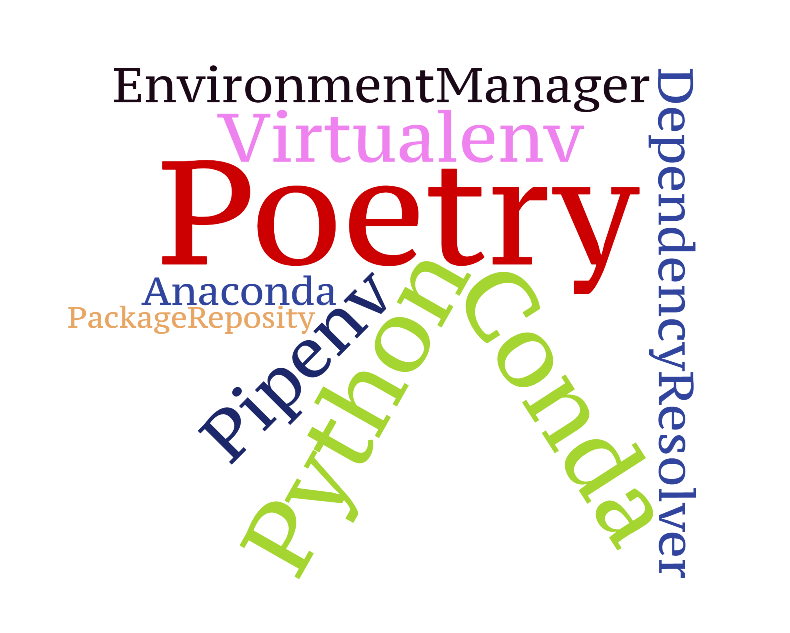
\includegraphics[width=\textwidth,height=5cm,keepaspectratio]{envinroments.png} 
            \end{figure}
        \end{column}
    \end{columns}
\end{frame}

\begin{frame}[t]{The "Lock File" Concept}
    \framesubtitle{Technically enforcing reproducibility}
    \vspace*{-0.5cm}
    \begin{columns}[T,onlytextwidth]
        \begin{column}{0.55\textwidth}
            \textbf{The Challenge}:
            You ask for \texttt{pandas}. It needs \texttt{numpy}, \texttt{pytz}, etc.
            Tomorrow, a new version of \texttt{numpy} is released and breaks your code.

            \textbf{The Solution}: Locking.
            \begin{itemize}
                \item \textbf{Manifest} (\texttt{pyproject.toml}): Abstract requirements ("I need pandas roughly version 2.0").
                \item \textbf{Lock File}: Concrete Snapshot. Contains exact versions and cryptographic hashes of \textit{all} transitive dependencies.
            \end{itemize}
            \textit{Rule}: Always commit the lock file to Git!
        \end{column}
        \begin{column}{0.43\textwidth}
            \begin{figure}[H]
                \centering
                \resizebox{\linewidth}{!}{
                \begin{tikzpicture}[
                    node distance=3cm,
                    file/.style={rectangle, draw, fill=white, drop shadow, minimum width=2.2cm, minimum height=2.5cm, align=left, font=\scriptsize, rounded corners}
                ]
                    \node[file, fill=blue!5] (toml) {\textbf{Manifest}\\pandas $\ge$ 2.0\\flask = *};
                    \node[file, fill=green!10, right of=toml] (lock) {\textbf{Lock File}\\pandas==2.1.0\\numpy==1.26.0\\flask==3.0.0\\werkzeug==3.0.1\\(sha256:7f8a...)};

                    \draw[->, thick, shorten >=2pt, shorten <=2pt] (toml) -- node[above, font=\tiny, align=center]{Resolver\\(SAT Solver)} (lock);
                \end{tikzpicture}
                }
                \caption{Resolution Process}
            \end{figure}
        \end{column}
    \end{columns}
\end{frame}

\begin{frame}[t]{Tool 1: uv (The Speedster)}
    \framesubtitle{Modern replacement for pip, venv, and pip-tools}
    \vspace*{-0.5cm}
    \begin{columns}[T,onlytextwidth]
        \begin{column}{0.60\textwidth}
            \textbf{Core Features}:
            \begin{itemize}
                \item Written in \textbf{Rust}. Extremely fast (10-100x faster than pip).
                \item Unified tool: Manages python versions, virtual envs, and packages.
                \item \textbf{Deterministic}: Generates \texttt{uv.lock} for reproducible builds.
            \end{itemize}
            
            \textbf{Best For}:
            \begin{itemize}
                \item CI/CD Pipelines (caches are heavily optimized).
                \item Rapid prototyping and scripting.
            \end{itemize}
        \end{column}
        \begin{column}{0.38\textwidth}
            \begin{figure}[H]
                \centering
                % SUGGESTION: Bar chart comparing installation time (pip vs poetry vs uv)
                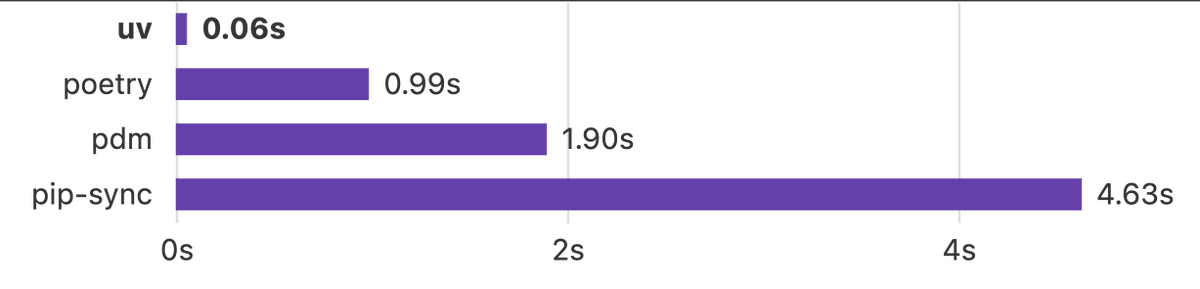
\includegraphics[width=\textwidth,height=4cm,keepaspectratio]{uv.png} 
                \caption*{Benchmark: Package Installation Time}
            \end{figure}
        \end{column}
    \end{columns}
\end{frame}

\begin{frame}[t]{Why Speed Matters?}
    \framesubtitle{CI/CD Costs \& Developer Experience}
            \textbf{1. Developer Flow}:
            \begin{itemize}
                \item Waiting for dependencies breaks mental context.
                \item "Context switching" is expensive.
            \end{itemize}

            \textbf{2. Continuous Integration (CI)}:
            \begin{itemize}
                \item Clean install happens on \textit{every} Pull Request.
                \item \textbf{Scenario}: 10 devs, 5 PRs/day.
                \begin{itemize}
                    \item Tool A (5 min): 250 mins/day wasted.
                    \item Tool B (10 sec): 8 mins/day wasted.
                \end{itemize}
            \end{itemize}
\end{frame}

\begin{frame}[fragile,t]{Tool 2: Poetry (The Developer Standard)}
    \framesubtitle{Dependencing Management \& Packaging}
    \begin{columns}[T,onlytextwidth]
        \begin{column}{0.60\textwidth}
            \textbf{Core Features}:
            \begin{itemize}
                \item Uses \texttt{pyproject.toml} (PEP 518 standard).
                \item \textbf{Strict Resolver}: Guarantees no conflicting dependencies.
                \item Handles packaging and publishing to PyPI.
            \end{itemize}
            
            \textbf{Best For}:
            \begin{itemize}
                \item Developing Python Libraries.
                \item Projects where strict dependency logic is crucial.
            \end{itemize}
        \end{column}
        \begin{column}{0.38\textwidth}
            \scriptsize \textbf{\texttt{pyproject.toml}}:
            \begin{lstlisting}[language=Python, basicstyle=\tiny\ttfamily, keywordstyle=\color{blue}, stringstyle=\color{green!50!black}, frame=single, backgroundcolor=\color{white}]
[tool.poetry]
name = "my-lib"
version = "0.1.0"

[tool.poetry.dependencies]
python = "^3.10"
numpy = "^1.26"
pandas = ">=2.0"

[tool.poetry.group.dev]
pytest = "^7.4"
            \end{lstlisting}
        \end{column}
    \end{columns}
\end{frame}

\begin{frame}[t]{Tool 3: Conda (The Scientific Heavyweight)}
    \framesubtitle{Binary Package Management}
            \textbf{Core Features}:
            \begin{itemize}
                \item **Language Agnostic**: Installs Python, C++, CUDA, R, etc.
                \item **Pre-compiled Binaries**: avoiding "GCC compilation failed" errors.
                \item Solves deep system dependencies (e.g., specific glibc versions).
            \end{itemize}
            
            \textbf{Best For}:
            \begin{itemize}
                \item Data Science \& ML (PyTorch, TensorFlow).
                \item Working with non-Python libraries (GDAL, FFMPEG).
            \end{itemize}
\end{frame}

\begin{frame}[t]{Tool 4: Pixi (The Modern Hybrid)}
    \framesubtitle{Conda power with Rust speed}
            \textbf{Core Features}:
            \begin{itemize}
                \item Uses \textbf{conda-forge} ecosystem (access to all binary packages).
                \item \textbf{Project-Local}: Installs everything in \texttt{.pixi} folder (no global env pollution).
                \item Works like \texttt{npm} or \texttt{cargo}. Cross-platform lock-files.
            \end{itemize}
            
            \textbf{Best For}:
            \begin{itemize}
                \item Reproducible ML Projects (Sharing code that "just works").
                \item Robotics (installing ROS packages via boa/conda).
            \end{itemize}
\end{frame}

\begin{frame}[t]{Docker: Shipping the Computer}
    \framesubtitle{Solving the "Matrix from Hell"}
    \vspace*{-0.5cm}
    \textbf{Concept}: Package your application with everything it needs to run (Code + Runtime + System Tools + System Libs).
    \begin{columns}[T,onlytextwidth]
        \begin{column}{0.55\textwidth}

            
            \textbf{Why?}
            \begin{itemize}
                \item Solves "Matrix of Hell" (OS $\times$ App version).
                \item Immutable Infrastructure: The image you test is the image you deploy.
            \end{itemize}
        
            \textbf{Robotics/ML Specifics}:
            \begin{itemize}
                \item \textbf{GPU Access}: nvidia-container-toolkit
                \item \textbf{GUI}: X11 forwarding to see \texttt{rviz} or plots.
                \item \textbf{Hardware}: \texttt{--network host}, \texttt{--privileged}.
            \end{itemize}
        \end{column}
        \begin{column}{0.45\textwidth}
            \begin{figure}[H]
                \centering
                % SUGGESTION: "Virtual Machine vs Docker Container" architecture diagram
                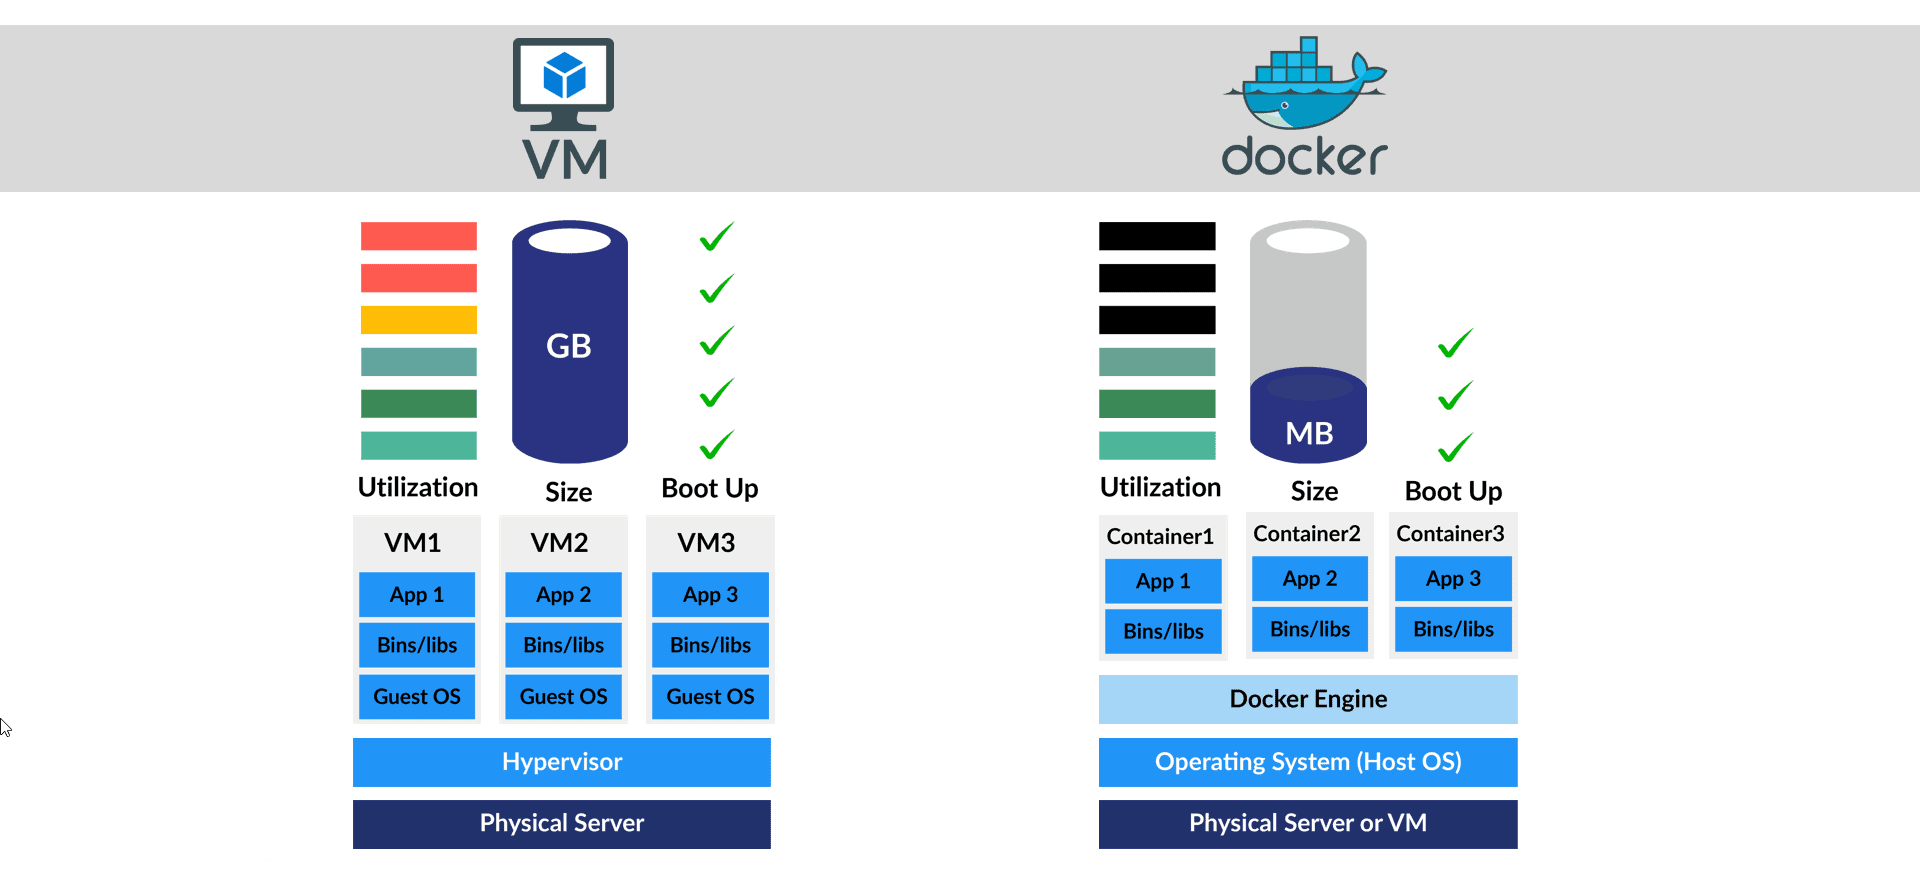
\includegraphics[width=\textwidth,height=5cm,keepaspectratio]{docker_vm.png} 
            \end{figure}
        \end{column}
    \end{columns}
\end{frame}

\begin{frame}[t]{Docker: Multi-stage Builds}
    \vspace*{-0.5cm}
    \textbf{Idea}: Use intermediate images to build items, copy only artifacts to the final image.

    \textbf{Example}:
    \begin{itemize}
        \item \textit{Stage 1 (Builder)}: Large image with \texttt{gcc}, \texttt{cmake}, headers. Compiles code. (Size: 2GB)
        \item \textit{Stage 2 (Runtime)}: Minimal OS + Binary. (Size: 100MB)
    \end{itemize}
    
    \begin{columns}[T,onlytextwidth]
        \begin{column}{0.48\textwidth}
            \textbf{Pros}:
            \begin{itemize}
                \item Minimal prod image size.
                \item Security (no compilers/keys in prod).
            \end{itemize}
        \end{column}
        \begin{column}{0.48\textwidth}
             \textbf{Cons}:
            \begin{itemize}
               \item Dockerfile complexity.
                \item Harder to debug build issues in prod image.
            \end{itemize}
        \end{column}
    \end{columns}
\end{frame}

\begin{frame}[t]{Orchestration: Docker Compose}
    \framesubtitle{Managing Multi-Container Robotics Systems}
    \vspace*{-0.5cm}
    \begin{columns}[T,onlytextwidth]
        \begin{column}{0.65\textwidth}
            \textbf{Why?}: Managing multiple containers with CLI flags is painful.
            
            \textbf{Role}: "Infrastructure as Code" for local development. Define services, networks, and volumes in one YAML file.
            
            \textbf{Microservices in Robotics (ROS 2)}:
            \begin{itemize}
                \item \textit{Drivers Container}: Hardware access.
                \item \textit{Perception Container}: PyTorch/CUDA environment.
                \item \textit{Planning Container}: C++ environment.
            \end{itemize}
            \textit{Benefit}: Isolation. Crash in Vision node doesn't kill the Motor controller.
        \end{column}
        \begin{column}{0.33\textwidth}
            \vspace*{-1.5cm}
            \begin{figure}[H]
                \centering
                \resizebox{!}{0.8\textheight}{
                \begin{tikzpicture}[
                    node distance=2.2cm,
                    container/.style={rectangle, draw=black!60, fill=blue!10, text width=5.5em, text centered, rounded corners=4pt, minimum height=3em, font=\scriptsize\bfseries},
                    arrow/.style={-stealth, thick, draw=black!70}
                ]
                    \node[container] (drivers) {Drivers\\(Camera)};
                    \node[container, below of=drivers] (percep) {Perception\\(GPU/AI)};
                    \node[container, below of=percep] (logic) {Control\\(Planner)};

                    \draw[arrow] (drivers) -- node[right, font=\tiny] {/image\_raw} (percep);
                    \draw[arrow] (percep) -- node[right, font=\tiny] {/detections} (logic);

                \end{tikzpicture}
                }
            \end{figure}
        \end{column}
    \end{columns}
\end{frame}

\begin{frame}[t]{Summary: Strategy Selection}
    \begin{columns}[T,onlytextwidth]
        \begin{column}{0.55\textwidth}
            \begin{itemize}
                \setlength\itemsep{0.5em}
                \item Just a script / Speed matter? $\rightarrow$ \textbf{uv}
                \item Developing Python Library? $\rightarrow$ \textbf{Poetry}
                \item Data Science with complex binaries? $\rightarrow$ \textbf{Pixi} (or Conda)
                \item Need to share with others / Deploy? $\rightarrow$ \textbf{Docker}
                \item Multiple services? $\rightarrow$ \textbf{Docker Compose}
            \end{itemize}
        \end{column}
        \begin{column}{0.43\textwidth}
            \vspace*{-1.2cm}
            \begin{figure}[H]
                \centering
                \resizebox{\linewidth}{!}{
                \begin{tikzpicture}[
                    node distance=1.8cm,
                    auto,
                    decision/.style={diamond, aspect=1.5, draw, fill=yellow!20, text width=4em, text centered, font=\scriptsize},
                    block/.style={rectangle, draw, fill=blue!10, text width=4.5em, text centered, rounded corners, minimum height=2em, font=\bfseries\scriptsize},
                    line/.style={draw, -stealth, thick}
                ]
                    \node [decision] (type) {Task?};
                    
                    \node [block, below of=type, xshift=-2.5cm] (uv) {uv};
                    \node [block, below of=type] (poetry) {Poetry};
                    \node [block, below of=type, xshift=2.5cm] (pixi) {Pixi};
                    
                    % Edges from Task
                    \path [line] (type) -| node [above, near start, font=\tiny] {Script} (uv);
                    \path [line] (type) -- node [right, font=\tiny] {Lib} (poetry);
                    \path [line] (type) -| node [above, near start, font=\tiny] {Systems} (pixi);
                    
                    \node [decision, below of=poetry, node distance=2.5cm] (deploy) {Deploy?};
                    
                    % Edges to Deploy
                    \path [line] (uv) |- (deploy);
                    \path [line] (poetry) -- (deploy);
                    \path [line] (pixi) |- (deploy);
                    
                    \node [block, below of=deploy, xshift=-1.5cm, fill=green!10] (docker) {Docker};
                    \node [block, below of=deploy, xshift=1.5cm, fill=green!10] (compose) {Compose};
                    
                    % Edges from Deploy
                    \path [line] (deploy) -| node [above, near start, font=\tiny] {Single} (docker);
                    \path [line] (deploy) -| node [above, near start, font=\tiny] {Multi} (compose);
                \end{tikzpicture}
                }
                \caption*{Decision Flowchart}
            \end{figure}
        \end{column}
    \end{columns}
\end{frame}


\fbckg{fibeamer/figs/last_page.png}
\frame[plain]{}

\end{document}